\chapter{Testarea Sistemului și Analiza Performanțelor \label{testare}}

Validarea prototipului hardware și software reprezintă etapa critică în confirmarea succesului metodologiei de proiectare propuse. Acest capitol prezintă metodologia de testare utilizată, instrumentele de măsură și rezultatele experimentale obținute, vizând atât performanțele etajelor analogice, cât și funcționalitatea procesării digitale de semnal.

\section{Metodologia de testare și setup-ul experimental}

Măsurătorile au fost efectuate într-un regim de buclă închisă (\textit{loopback}), utilizând o interfață audio profesională externă pentru generarea semnalelor de test și achiziția răspunsului sistemului. Software-ul principal utilizat pentru analiza spectrală și generarea sweep-urilor de frecvență a fost \textbf{Room EQ Wizard (REW)}.

Setup-ul experimental include următoarele instrumente:
\begin{itemize}
    \item \textbf{Interfață audio:} Focusrite Scarlett pentru generare semnal și monitorizare;
    \item \textbf{Osciloscop digital:} Pentru vizualizarea formelor de undă;
    \item \textbf{Software:} REW pentru măsurători de răspuns în frecvență și SigmaStudio pentru controlul DSP-ului în timp real.
\end{itemize}

\section{Validarea interfeței de intrare cu câștig comutabil}

Un obiectiv central al testării a fost verificarea preciziei etajului de intrare (\textit{switched-gain preamp}). S-a urmărit demonstrarea capacității circuitului de a scala standardele de nivel $+4\text{ dBu}$ ($1.228\text{ V}_{rms}$) și $-10\text{ dBV}$ ($0.316\text{ V}_{rms}$) la valoarea țintă de aproximativ $1\text{ V}_{rms}$, indiferent de tipul conexiunii (echilibrată sau neechilibrată).

\subsection{Testarea în regim Echilibrat}
Prima serie de măsurători a vizat conectorii de tip Combo în modul diferențial. Rezultatele sunt prezentate în Figura \ref{fig:scope_bal}.

\begin{figure}[htbp]
    \centering
    \begin{subfigure}{0.48\textwidth}
        \centering
        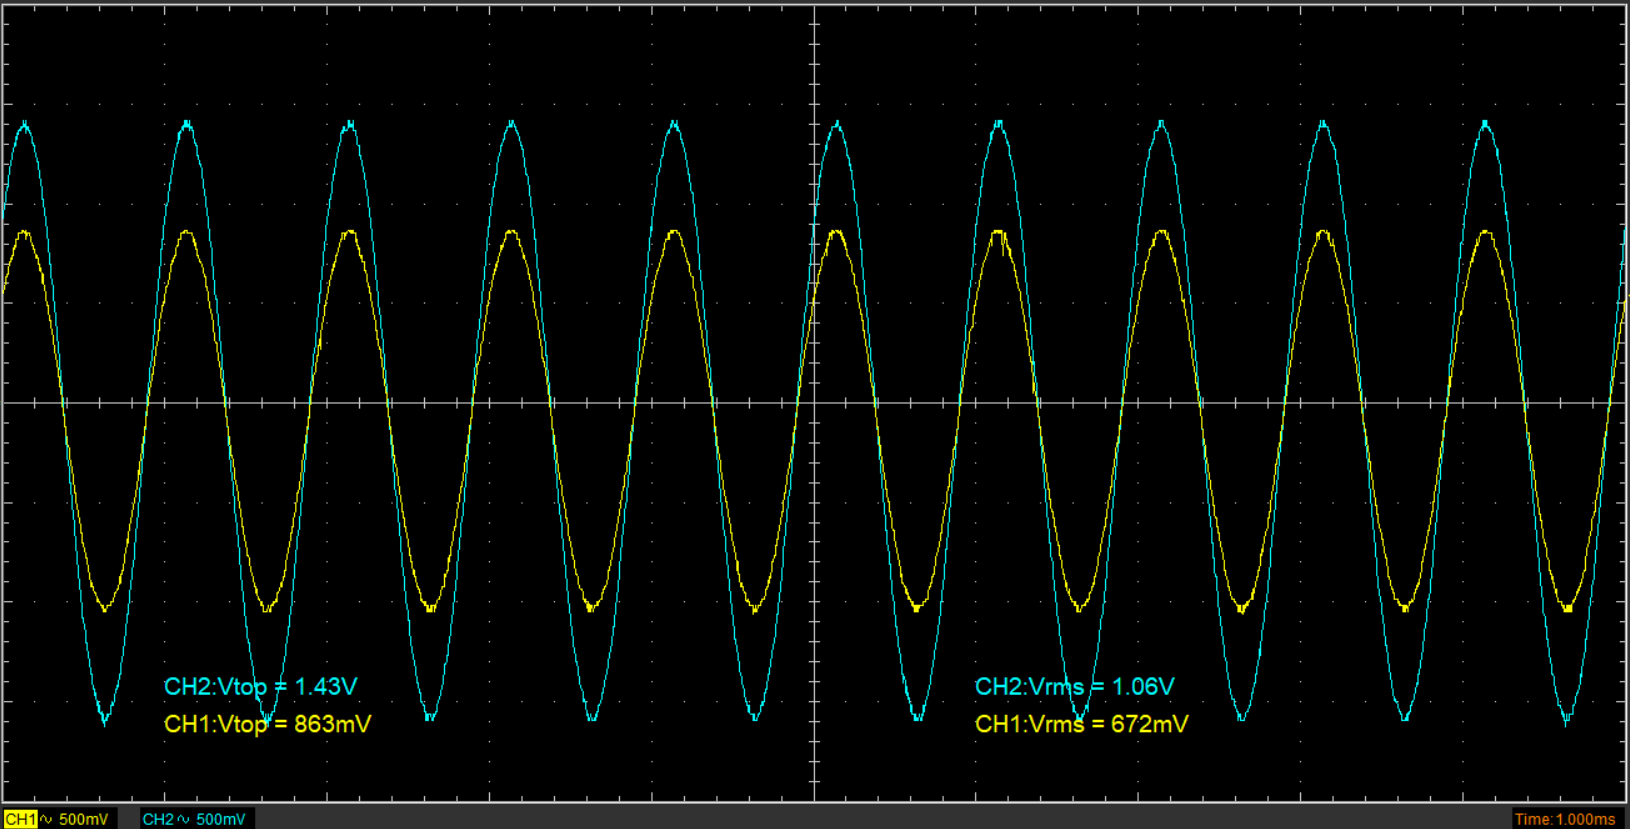
\includegraphics[width=\textwidth]{figuri/Preamp_4dBU_Balanced.png}
        \caption{Low Gain (+4 dBu).}
    \end{subfigure}
    \hfill
    \begin{subfigure}{0.48\textwidth}
        \centering
        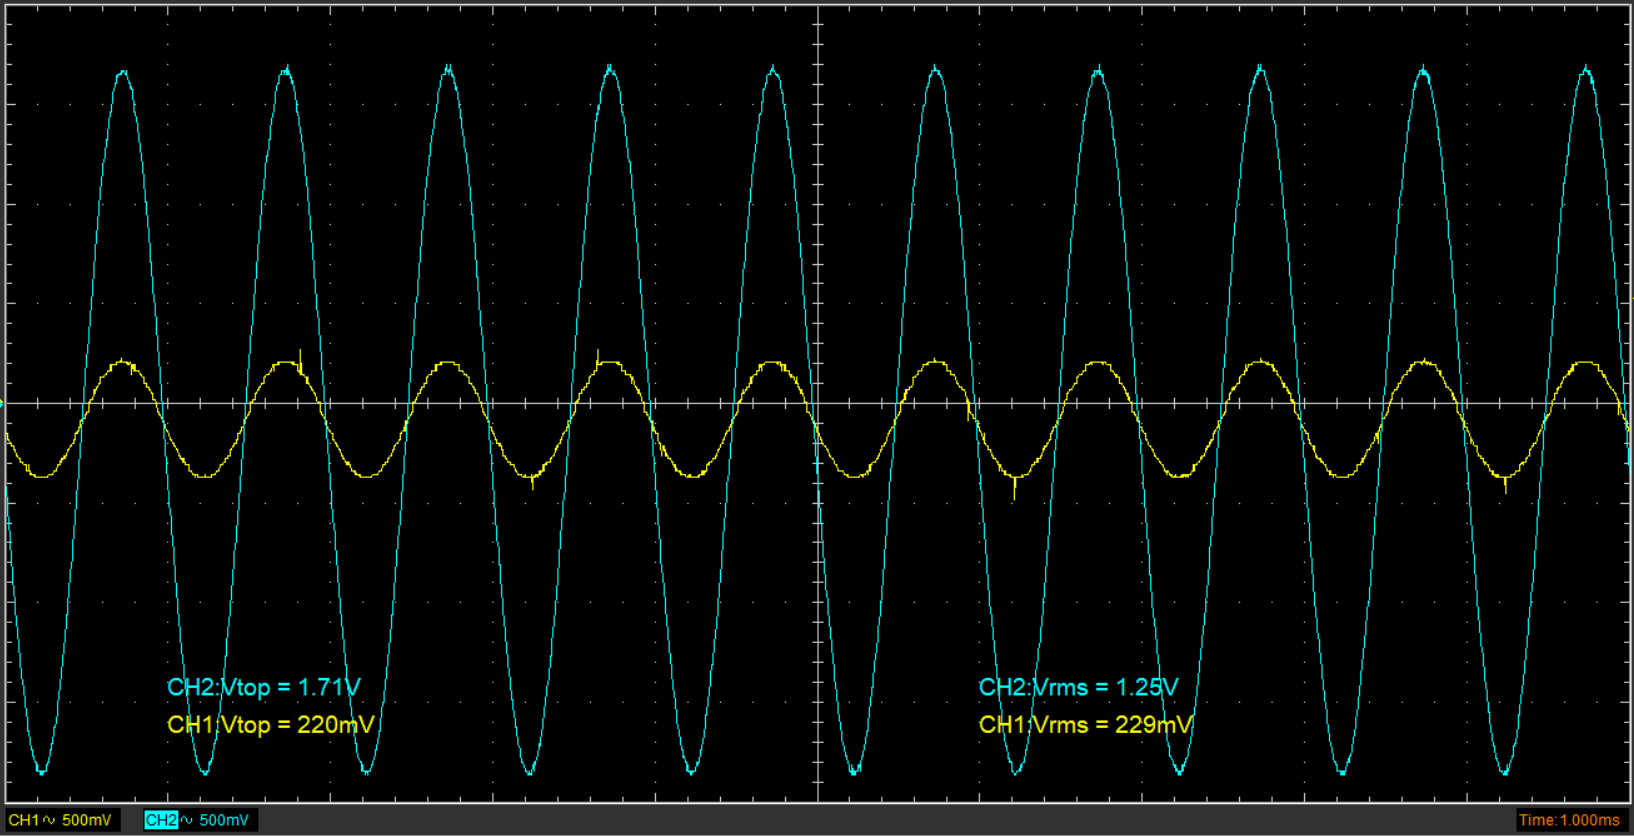
\includegraphics[width=\textwidth]{figuri/Preamp_10dBV_Balanced.png}
        \caption{High Gain (-10 dBV).}
    \end{subfigure}
    \caption{Capturi de osciloscop pentru intrarea echilibrată: CH1 (galben) - intrare Cald, CH2 (albastru) - ieșire preamp.}
    \label{fig:scope_bal}
\end{figure}

Pentru regimul \textit{Low Gain}, s-a obținut un câștig experimental de $G_{bal,low} = 0.788$. În regimul \textit{High Gain}, s-a obținut $G_{bal,high} = 2.73$.

\subsection{Testarea în regim Neechilibrat}
A doua serie de măsurători a utilizat intrarea dedicată pentru semnale neechilibrate. Rezultatele sunt prezentate în Figura \ref{fig:scope_unbal}.

\begin{figure}[htbp]
    \centering
    \begin{subfigure}{0.48\textwidth}
        \centering
        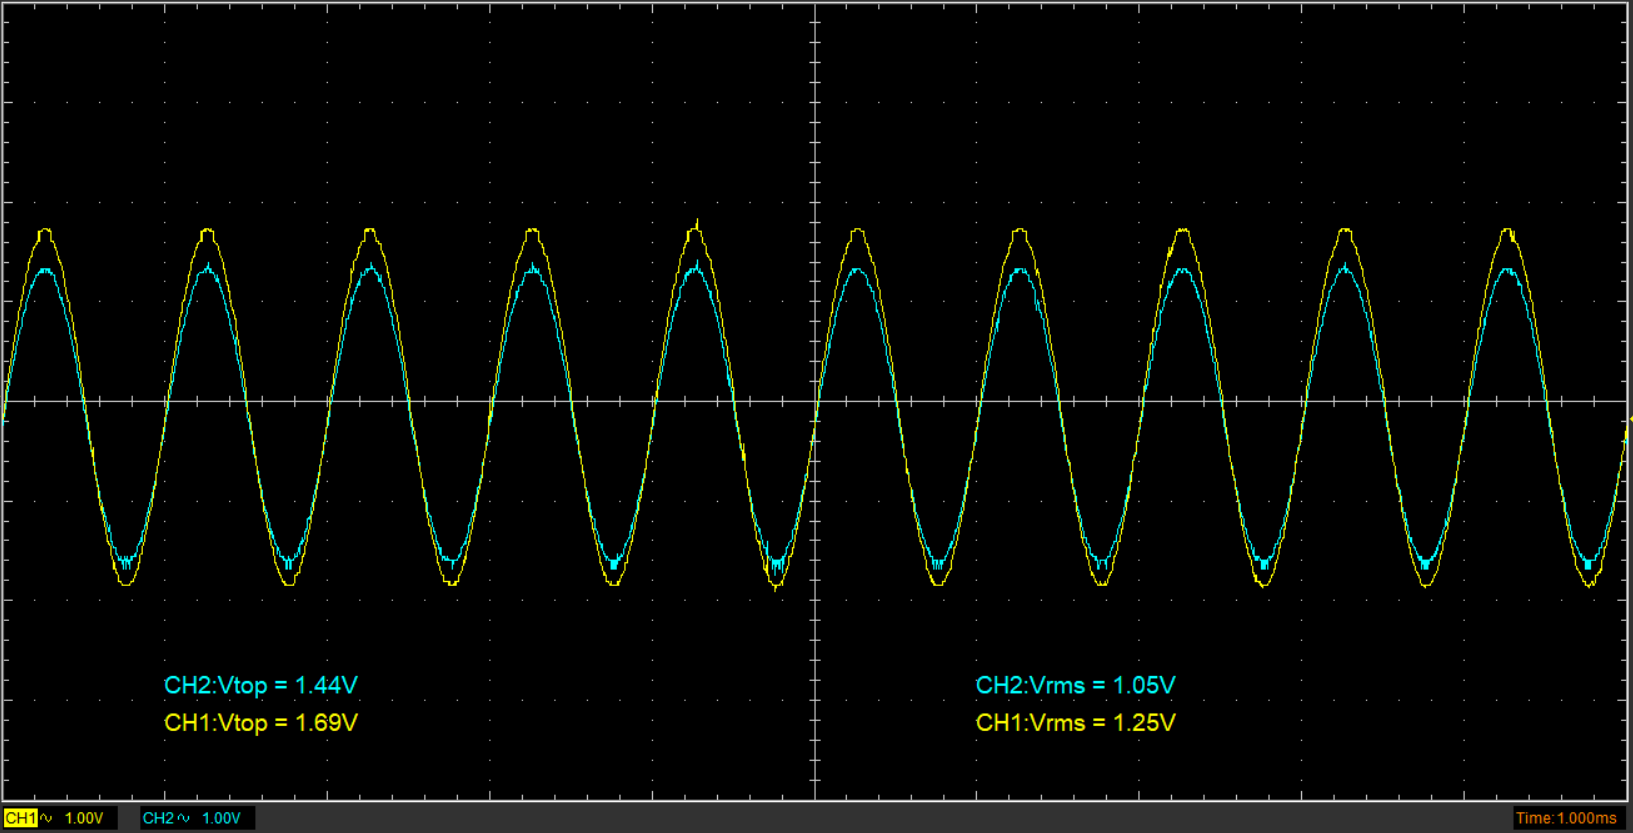
\includegraphics[width=\textwidth]{figuri/Preamp_4dBU_Unbalanced.png}
        \caption{Low Gain (+4 dBu).}
    \end{subfigure}
    \hfill
    \begin{subfigure}{0.48\textwidth}
        \centering
        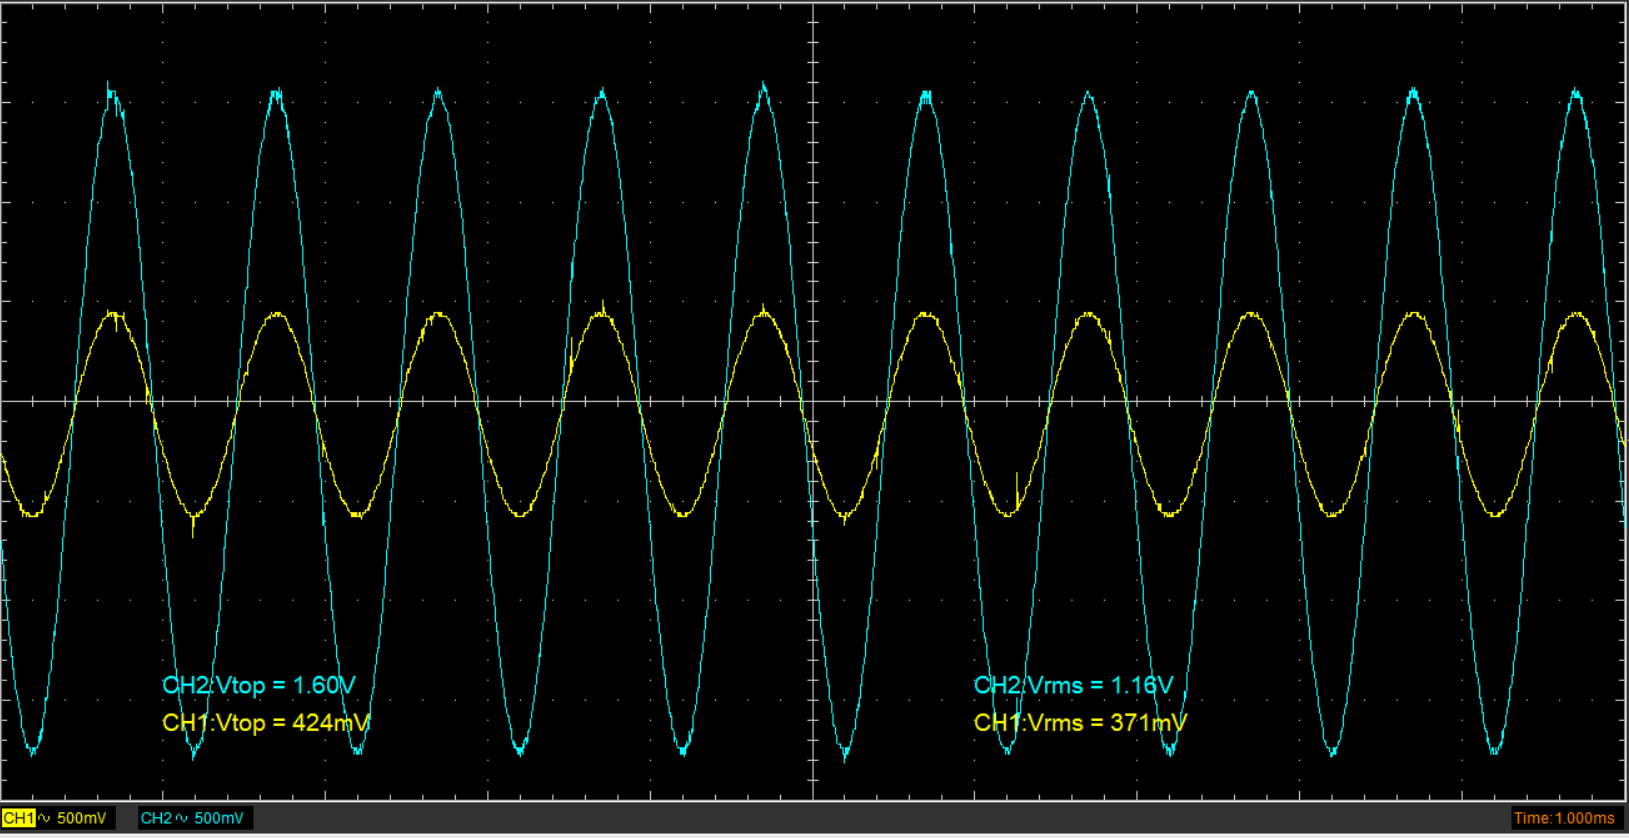
\includegraphics[width=\textwidth]{figuri/Preamp_10dBV_Unbalanced.png}
        \caption{High Gain (-10 dBV).}
    \end{subfigure}
    \caption{Capturi de osciloscop pentru intrarea neechilibrată: CH1 (galben) - intrare , CH2 (albastru) - ieșire preamp.}
    \label{fig:scope_unbal}
\end{figure}

În acest mod, precizia a fost remarcabilă. Pentru \textit{Low Gain}, s-a măsurat un câștig de $G_{unbal,low} = 0.84$ (abatere de $2.4\%$ față de $0.82$ teoretic). Pentru \textit{High Gain}, s-a măsurat un câștig de $G_{unbal,high} = 3.12$, reprezentând o eroare neglijabilă de $0.3\%$ față de valoarea teoretică de $3.13$.

\subsection{Sinteza rezultatelor}
Datele obținute sunt centralizate în Tabelul \ref{tab:masuratori_gain}.

\begin{table}[htbp]
    \centering
    \caption{Rezultate experimentale: Maparea nivelurilor nominale.}
    \label{tab:masuratori_gain}
    \begin{tabular}{@{}ccccc@{}}
    \toprule
    \textbf{Sursă} & \textbf{Standard} & \textbf{Mod} & \textbf{Gain ($G$)} & \textbf{V$_{out,calc}$ [V$_{rms}$]} \\ \midrule
    Balanced & Professional & Low Gain & $0.788$ & $0.968$ \\
    Balanced & Consumer & High Gain & $2.730$ & $0.863$ \\
    Unbalanced & Professional & Low Gain & $0.840$ & $1.031$ \\
    Unbalanced & Consumer & High Gain & $3.126$ & $0.988$ \\
    \bottomrule
    \end{tabular}
\end{table}

Analiza rezultatelor confirmă validitatea topologiei proiectate. În toate cele patru scenarii, semnalul este adus în intervalul $0.85\text{--}1.05\text{ V}_{rms}$, asigurând utilizarea optimă a dinamicii ADC-ului.

\section{Răspunsul în frecvență al sistemului}

Măsurarea răspunsului în frecvență a fost realizată pentru a valida transparența hardware-ului și eficacitatea procesării digitale realizate în DSP.

\subsection{Regimul Bypass}
S-a încărcat o configurație neutră în procesorul ADAU1701. Rezultatele (Figura \ref{fig:freq_bypass}) indică un răspuns liniar în banda $20\text{ Hz} - 20\text{ kHz}$. Atenuările ușoare la capetele benzii sunt atribuite filtrelor de decuplare DC, însă rămân în parametrii de performanță acceptați pentru un sistem de înaltă fidelitate ($\pm 1.5\text{ dB}$).

\begin{figure}[htbp]
    \centering
    \begin{subfigure}{0.48\textwidth}
        \centering
        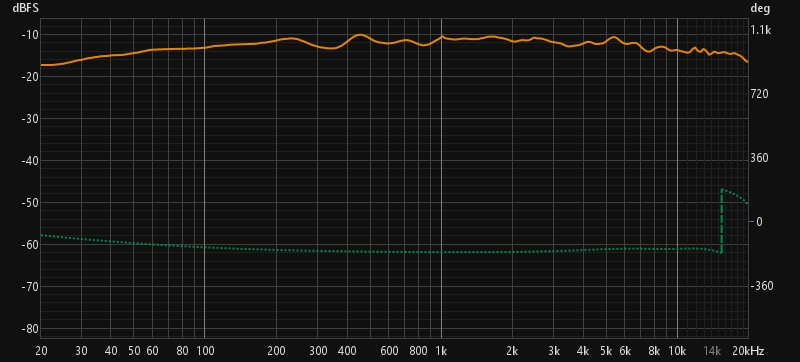
\includegraphics[width=\textwidth]{figuri/Balanced_4dBU_freq_Bypas.jpg}
        \caption{Balanced, +4 dBu.}
    \end{subfigure}
    \hfill
    \begin{subfigure}{0.48\textwidth}
        \centering
        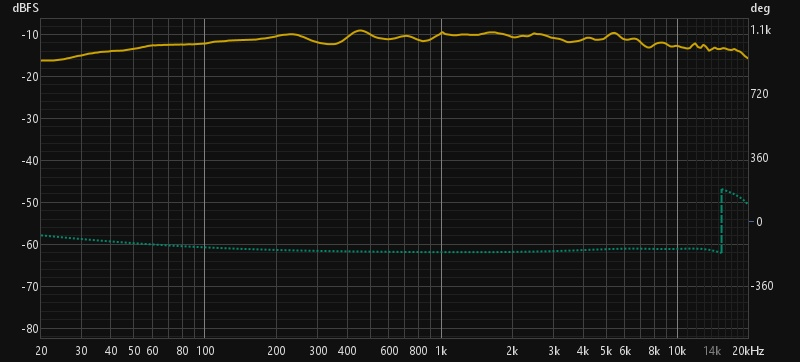
\includegraphics[width=\textwidth]{figuri/Balanced_10dBV_freq_Bypas.jpg}
        \caption{Balanced, -10 dBV.}
    \end{subfigure}
    
    \vspace{0.5cm}
    
    \begin{subfigure}{0.48\textwidth}
        \centering
        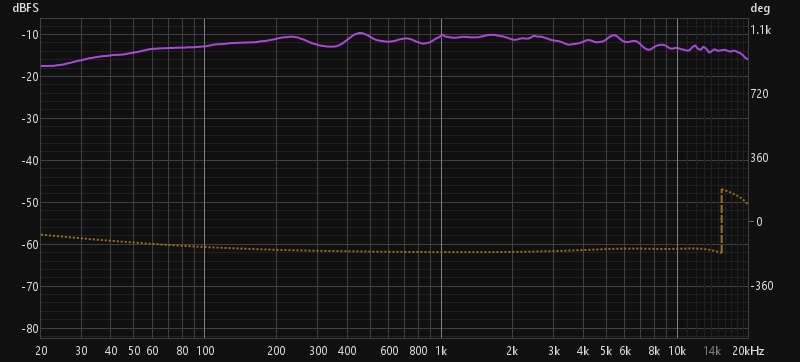
\includegraphics[width=\textwidth]{figuri/Unbalanced_4dBU_freq_Bypas.jpg}
        \caption{Unbalanced, +4 dBu.}
    \end{subfigure}
    \hfill
    \begin{subfigure}{0.48\textwidth}
        \centering
        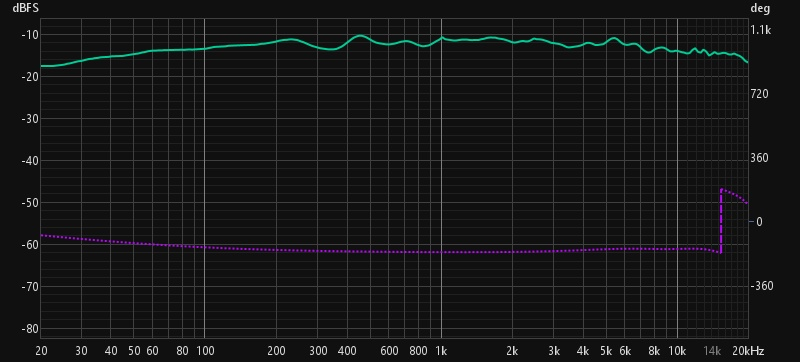
\includegraphics[width=\textwidth]{figuri/Unbalanced_10dBV_freq_Bypas.jpg}
        \caption{Unbalanced, -10 dBV.}
    \end{subfigure}
    \caption{Răspunsul în frecvență (magnitudine și fază) în regim Bypass pentru diverse configurații de intrare.}
    \label{fig:freq_bypass}
\end{figure}

\subsection{Regimul cu procesare activă}
Pentru a demonstra controlul precis oferit de DSP, s-a implementat în SigmaStudio un filtru trece-bandă (\textit{Bandpass Filter}) centrat pe frecvența de $1\text{ kHz}$ (Figura \ref{fig:sigma_sch}). Alegerea acestui tip de filtru a fost motivată de necesitatea de a observa clar atenuarea atât a frecvențelor joase, cât și a celor înalte, oferind o confirmare vizuală imediată a integrității lanțului de procesare.

Configurația filtrului a utilizat un ordin 2 (filtru de tip biquad), cu un factor de calitate $Q = 1.41$, vizând o curbă de răspuns netedă în banda de trecere. Procesul de implementare în SigmaStudio a presupus rutarea semnalului de intrare prin blocul \textit{General Second-Order Filter}.

\begin{figure}[htbp]
    \centering
    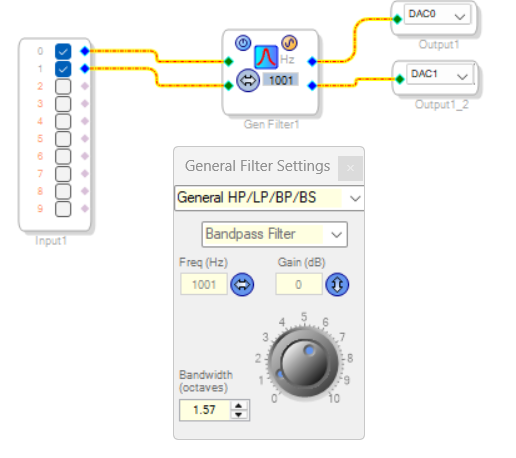
\includegraphics[width=0.4\textwidth]{figuri/sigma_studio_effect.png}
    \caption{Configurarea filtrului Bandpass în mediul SigmaStudio.}
    \label{fig:sigma_sch}
\end{figure}

Măsurătoarea corespunzătoare (Figura \ref{fig:freq_effect}) confirmă aplicarea corectă a filtrului, cu o atenuare pronunțată în afara benzii de trecere, validând astfel funcționarea algoritmilor de procesare în timp real.

\begin{figure}[htbp]
    \centering
    \begin{subfigure}{0.48\textwidth}
        \centering
        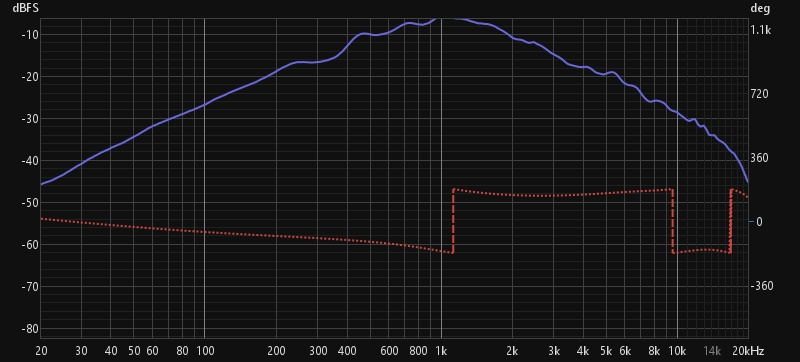
\includegraphics[width=\textwidth]{figuri/Balanced_4dBU_effect.jpg}
        \caption{Balanced, +4 dBu.}
    \end{subfigure}
    \hfill
    \begin{subfigure}{0.48\textwidth}
        \centering
        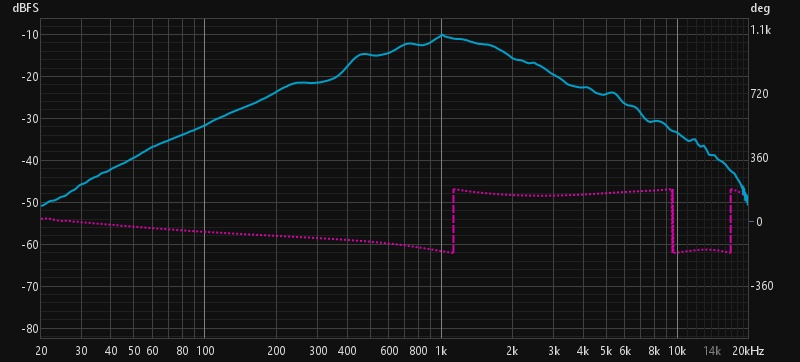
\includegraphics[width=\textwidth]{figuri/Unbalanced_4dBU_freq_effect.jpg}
        \caption{Unbalanced, +4 dBu.}
    \end{subfigure}
    \caption{Răspunsul în frecvență al sistemului cu filtrul Bandpass activat.}
    \label{fig:freq_effect}
\end{figure}

Această etapă de testare confirmă faptul că infrastructura software de control (SigmaStudio) comunică bidirecțional cu hardware-ul prin interfața USBi, permițând ajustări parametrice instantanee care se reflectă direct în performanța acustică a sistemului.

\section{Analiza performanțelor etajului de intrare}

Dincolo de răspunsul în frecvență, calitatea unui sistem audio este definită de capacitatea de respingere a zgomotului de mod comun, raportul semnal-zgomot și distorsiunile armonice introduse.

\subsection{Common Mode Rejection Ratio (CMRR)}
Măsurarea CMRR-ul a fost efectuată prin injectarea unui semnal identic pe ambele intrări ale etajului balansat (Hot și Cold unite). În Figura \ref{fig:cmrr_meas} este prezentată comparația între gain-ul diferențial și cel de mod comun.

\begin{figure}[htbp]
    \centering
    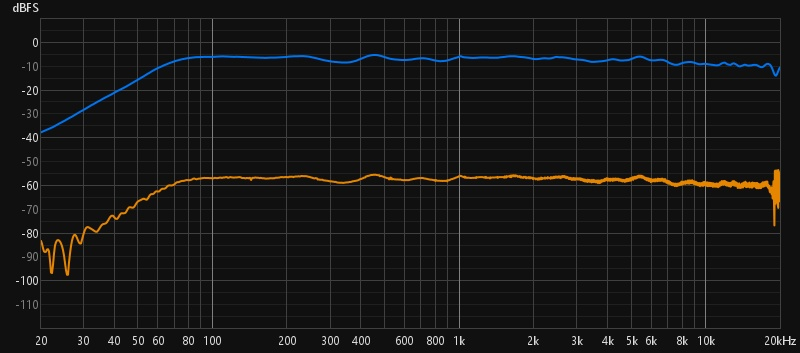
\includegraphics[width=0.8\textwidth]{figuri/cmmr.jpg}
    \caption{Măsurătoare CMRR în REW: Curba albastră (semnal diferențial), Curba portocalie (semnal de mod comun).}
    \label{fig:cmrr_meas}
\end{figure}

S-a obținut graficul din Figura \ref{fig:cmrr_final}, care indică o valoare medie a CMRR-ului de aproximativ $50.3\text{ dB}$ în banda audio utilă. Această performanță este considerată foarte bună pentru un montaj realizat pe perfboard, fiind limitată principal de toleranța de $1\%$ a rezistențelor utilizate în rețeaua diferențială.

\begin{figure}[htbp]
    \centering
    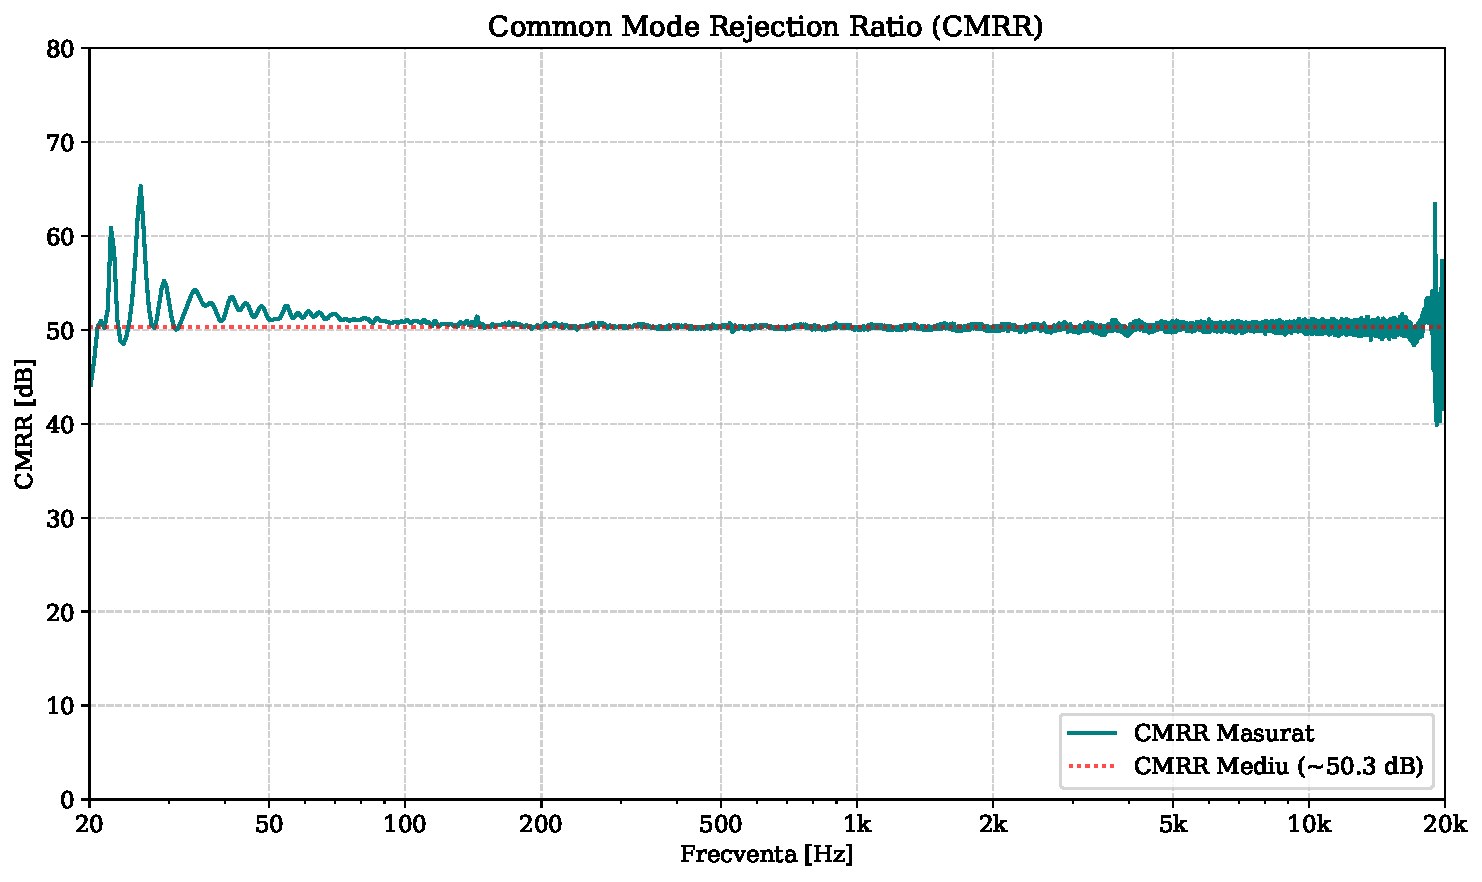
\includegraphics[width=0.8\textwidth]{figuri/cmrr_real.pdf}
    \caption{CMRR calculat în funcție de frecvență.}
    \label{fig:cmrr_final}
\end{figure}

\subsection{Zgomot și Distorsiuni (SNR și THD)}
Măsurătorile de zgomot (Figura \ref{fig:snr_meas}) și distorsiuni (Figura \ref{fig:thd_meas}) au fost realizate la o frecvență de test de $1\text{ kHz}$.

\begin{figure}[htbp]
    \centering
    \begin{subfigure}{0.48\textwidth}
        \centering
        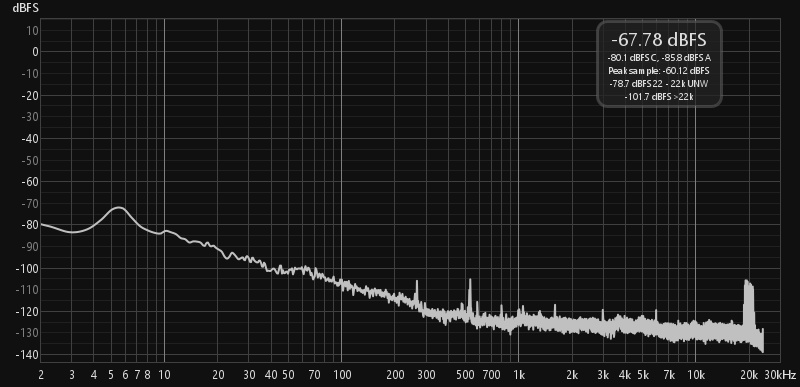
\includegraphics[width=\textwidth]{figuri/snr_balanced.jpg}
        \caption{Zgomot de fond - Balanced.}
    \end{subfigure}
    \hfill
    \begin{subfigure}{0.48\textwidth}
        \centering
        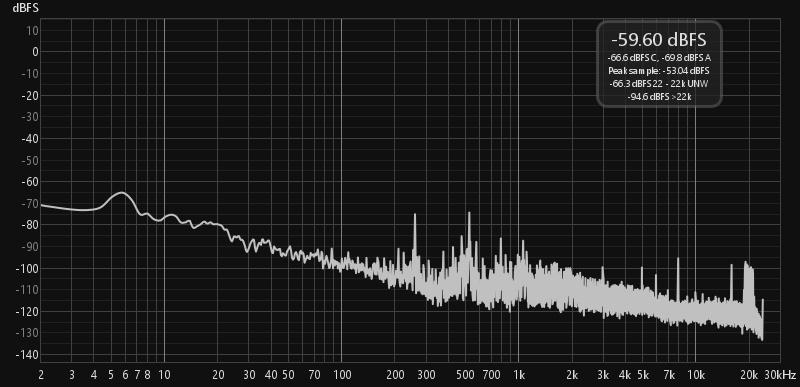
\includegraphics[width=\textwidth]{figuri/snr_unbalanced.jpg}
        \caption{Zgomot de fond - Unbalanced.}
    \end{subfigure}
    \caption{Analiza spectrală a zgomotului de fond (\textit{noise floor}).}
    \label{fig:snr_meas}
\end{figure}

Rezultatele pentru distorsiuni indică o performanță ridicată, cu o valoare THD de doar $0.0017\%$ în regim echilibrat. Raportul semnal-zgomot (SNR) obținut este de $59.8\text{ dB}$ pentru intrarea echilibrată și $50.4\text{ dB}$ pentru cea neechilibrată.

\begin{figure}[htbp]
    \centering
    \begin{subfigure}{0.48\textwidth}
        \centering
        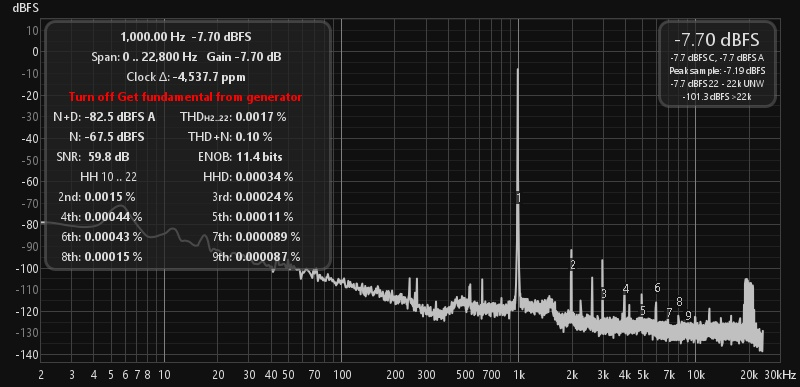
\includegraphics[width=\textwidth]{figuri/thd_balanced.jpg}
        \caption{THD - Balanced.}
    \end{subfigure}
    \hfill
    \begin{subfigure}{0.48\textwidth}
        \centering
        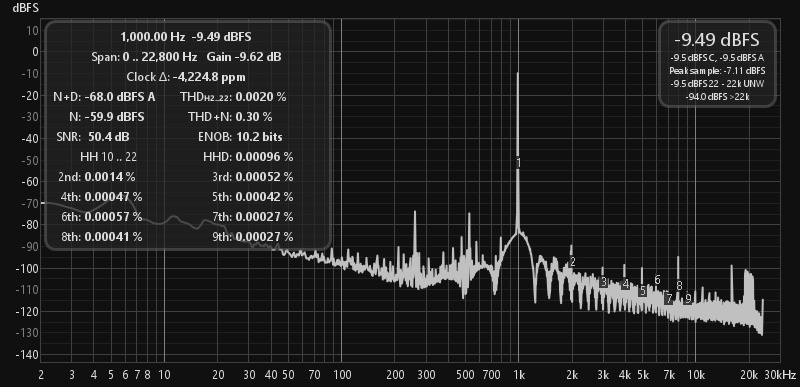
\includegraphics[width=\textwidth]{figuri/thd_unbalanced.jpg}
        \caption{THD - Unbalanced.}
    \end{subfigure}
    \caption{Măsurarea THD și SNR la $1\text{ kHz}$.}
    \label{fig:thd_meas}
\end{figure}

\section{Concluzii și direcții viitoare}

Proiectul a demonstrat realizarea unui sistem audio versatil, capabil de procesare digitală de înaltă rezoluție într-o structură compactă. Integrarea componentelor audio specializate și utilizarea unei mase virtuale stabile au permis obținerea unor performanțe solide, confirmate de măsurătorile experimentale.

Ca direcții viitoare de dezvoltare, se propune:
\begin{itemize}
    \item Proiectarea unui circuit imprimat (PCB) pe patru straturi cu planuri de masă dedicate pentru reducerea zgomotului de fond;
    \item Integrarea unei ecranări metalice interne pentru protecția împotriva interferențelor electromagnetice;
\end{itemize}
